\chapter{Implementation}

In this chapter, we explain the implementation plan and the work that has been done so far.

\section{Big Picture}

Indico is a complex product with many features. As a result, it as a large code base which is easily seen figure \ref{loccomp}\footnote{\href{https://www.ohloh.net/p/reddit}{Reddit on Ohloh}, \href{http://www.youtube.com/watch?v=MLM2acV\_1yo}{Yelp: Developing a Python service stack at Twitter University}, \href{https://www.ohloh.net/p/indico}{Indico on Ohloh}} in comparison to some popular services.

\begin{figure}[H]
  \caption{Line of code comparison between Reddit, Yelp and Indico}
  \centering
    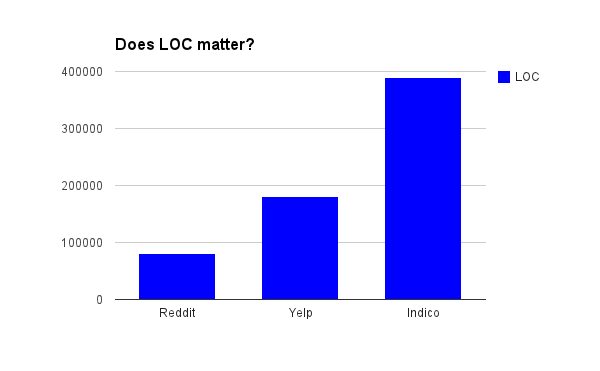
\includegraphics[scale=0.8]{6/figures/loccomp.png}
  \label{loccomp}
\end{figure}

This kind of complexity makes a database change a non-trivial operation that has to be done in step. Since we would like to see the result of our changes all the time, we need a working system. Therefore, the main database machinery, is first integrated and then each module is refactored into using the new database. At the same time, tests are being written to validate the behaviour of code. When a module is ready, after  careful testing, it is put in production. Other modules follow, being gradually refactored and moved to the production environment.

\section{Scope of Project}

When ZODB started to perform badly, incremental optimizations were done. For instance, Room Booking which enables location and room management, and reserving rooms for events, is one of the most complex and involving modules and has its own database (in CERN's production system). Since it's not very tightly integrated into the main database, it is a good starting point that allows the development team to gain experience in the frameworks and tools in question as well as in refactoring code to the new database. It also allows for more precise estimates to be established.

\section{Room Booking Schema}

Since we are going to use a RDBMS, a schema must be designed up-front.

We started inspecting database with external tools to get the object structure. However, ZODB being an object database, inspecting it is much harder, not only because the inspection tool needs run-time information about used classes but also because data is organized in a graph-like fashion. Even if three different tools are available for such job, none of them has shown to be stable and well-supported:
\begin{itemize}
  \item \texttt{zodbbrowser}
  \item \texttt{eye}
  \item \texttt{z3c.zodbbrowser} (unfinished GSOC\footnote{\href{http://www.google-melange.com/gsoc/homepage/google/gsoc2014}{Google Summer of Code}} project)
\end{itemize}

We have tried all of them but \textit{eye} was the most stable in our opinion and our experience. But even \textit{eye} wouldn't open our production database, which can be as big as 40 GB. Even a packed version won't be smaller than 15 GB.

The viewer could be patched, but the interaction with upstream developer showed to be slow. Te choice was, then, to use a subset of this database instead - data was loaded incrementally in order to find the rupture point. Next logical step was to analyse the mapped classes which wasn't an easy task, since some of the classes were as big as $\sim$2000 lines.

\begin{figure}[H]
  \caption{Room Booking Schema with CERN production data}
  \centering
    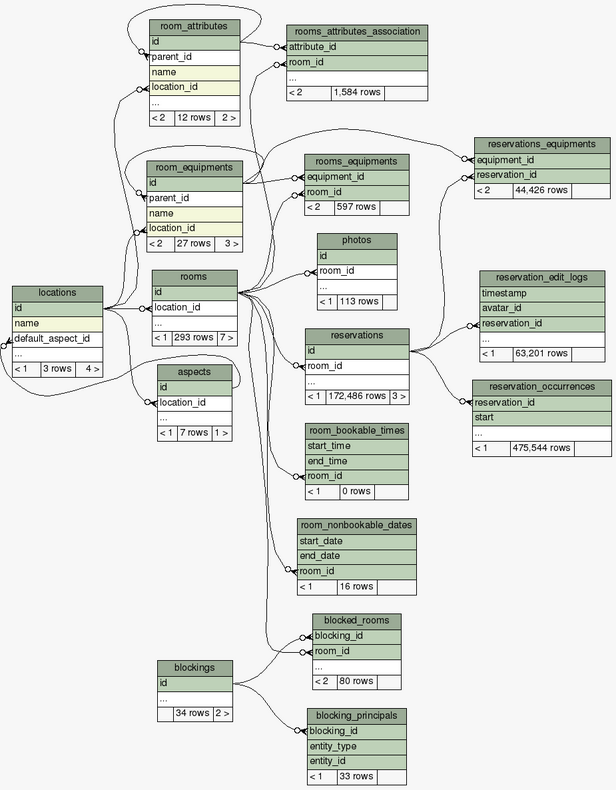
\includegraphics[scale=0.63]{6/figures/schema.png}
  \label{schema}
\end{figure}

Normalizing such a data set is a challenge, because most of the ZODB classes in question use the \textit{set}, \textit{list}, \textit{dictionary} data structures of Python and there are places where data is replicated within objects. They should be fully normalized into their own tables.

There are places which work nicely in small number of cases but don't scale:
\begin{itemize}
  \item Recurrence of room bookings: currently, there are only 6 options so their text representations and dates are calculated explicitly. Moreover, their implementation is not always precise. Some corner cases result in results that are not intuitive at all. Adding one more repetition type isn't easy so text and date generation needs some \textit{humanization} and a better computing algorithm.
  \item Location and Room attributes and equipments: These are replicated for each one, they all mean the same thing, though.
  \item Location and Room attributes and equipments: They have a hierarchy but this hierarchy is hard coded into the source code. Each level of this hierarchy is one list in room object, for instance.
  \item Location and Room attributes and equipments: Due to replication, there are inconsistencies. Rooms shouldn't be able to possess an equipment type that their corresponding location doesn't allow. However, ZODB's lack of schema or any other constraints makes it hard to enforce that.
  \item Booking occurrences are calculated on-the-fly. Booking objects keep track of the start and end data of the reservation as a whole, but the actual occurrences (in the case of recurring bookings) are generated in runtime, as are collisions checked.
\end{itemize}

The opportunity to re-design the DB schema brought the added benefit of being able to address these issues.

Finally, some helper scripts were implemented in order to easily generate a graph of the schema and a \textit{UML} diagram of classes. Understanding what is what from code inspection as a start may be a waste of time. Hopefully, these scripts will save some time in development, as they provide a high level view of the system that can be very useful. Fortunately, not all DB system suffer from the same issue as ZODB in terms of lack of tools: PostgreSQL, for instance, has pgAdmin, a powerful inspection tool.

\section{ORM - Object Relational Mapper}

A common problem that affects many modern web applications is that object orientation is not always easy to couple with relational models. An RDBMS is expecting tabular data. While a custom solution could be possible, fortunately there are libraries that provide this functionality out of the box:
\begin{itemize}
  \item SQLALchemy
  \item Django ORM
  \item pony
  \item peewee
  \item Storm
\end{itemize}

We have chosen SQLAlchemy. Django ORM would be an option, but it would be more appropriate if Indico used the Django web framework. Storm is developed at Canonical and has shown capabilities at the scale of Launchpad but other than that, there aren't many products. pony and peewee have a smaller user community and less features compared to SQLAlchemy.

SQLAlchemy is a very stable library approaching its $1.0$ major version and preferred by Mozilla, Nasa, OpenStack. Some of its nice features are:
\begin{itemize}
  \item Architecture: SQLAlchemy is composed of two layers, core and orm. ORM layer makes it easier to play with objects but more fine-grained control is tuned by the core layer.
  \item Declarative DDL, Data Definition Language.
  \item Unit of work: SQLAlchemy prevents excessive communication with the database, instead everything is put into queues and batched in one go.
  \item Powerful query generation: SQL construction from Python functions and expressions.
  \item Modular and extensible: Custom types, custom compilation of queries.
  \item Eager/Lazy loading and caching
\end{itemize}

Recently, the Flask web micro-framework was integrated into Indico. Before that, Indico had its own WSGI-compatible request handling and dispatching mechanism. Flask is now doing that job behind the scenes (even if there are some features in Flask that Indico is not yet using at their full extent). Flask-SQLAlchemy was chosen to provide tighter integration between Flask and SQLAlchemy.

\section{MVC - Model View Controller}

Many parts of Indico are not as modular as they should be. Every function related to one layer is put into the same file. Even though a lot of work is being done in order to improve that, some older files still have as much as $\sim$15000 lines. Navigating, understanding and editing it are difficult. Even text editor may sometimes freeze while editing such a big file.

Since we're refactoring, why don't we make our lives easier for the future? MVC (Model-View-Controller) pattern is a well-known software pattern that splits applications into interconnected parts. MVC enables separation between how data is represented within the system, how requests are handled and how data is shown to users.

Adapting the MVC pattern extensively in the new database-enabled code, in order to create  better and manageable software modules.

\section{Models}

We use SQLAlchemy and Flask-SQLAlchemy and their declarative DDL. 

Firstly, a base SQLAlchemy object that provides an interface with the database is put into \texttt{indico.core.db}. This object makes table and type primitives available.

Secondly, Models, which represent business objects, are put into their own separate files. Each class attribute is set to a column object of a specific type which is retrieved from the base \textit{DB} object.


At runtime, after the Flask application is created, the \textit{DB} object is imported and configured. Flask-SQLAlchemy comes with reasonable defaults. However, \textit{DB} is configured with values retrieved from the main Indico \textit{config} object, which itself contains Indico's default set of parameters for SQLAlchemy.

After getting an application context from the flask application and setting application of \textit{DB} object to this application, each model that is using SQLAlchemy should  be imported to resolve interdependence between models. At this time, we can drop existing database and/or create database. Models are ready to use.

\section{Distributed Queries}

ZODB can't be replaced from day to night so the chosen RDBMS and ZODB will have to coexist until full transition is achieved. Therefore, distributed queries must be supported. If one of databases returns an error, the transaction must be aborted and the connection state must be rolled back.

Once again, this problem could be solved with a "homemade" implementation, but, luckily, SQLAlchemy's \textit{session} object, ongoing transaction and local cache, is extensible enough to allow better than that. Therefore, adding /removing objects to/from the  \textit{session} may be done by the application developer while commit/roll-back is called by an extension. Moreover, ZODB's transaction module can manage external transactions in addition to its own ZODB transaction with a helper that provides a common ZODB interface. The architectures of these libraries nicely fit into Indico's own structured request handler hierarchy. Every request handler extends the \textit{base} request handler which is the only point where transactions are committed or rolled back.

To make this design possible, we use \textit{zope.sqlalchemy} which is a joint effort of ZODB and SQLAlchemy developers. Since only the base request handler in Indico deals with transaction logic, developers are not exposed to it.

Making \textit{base} request handler only responsible, developers aren't needed to deal with transaction logic any where else, they only manipulate objects, instead and \textit{base} request handler handles the rest because when a request has come, one thread-local \textit{session} is created and one transaction is started. Developer uses this \textit{session} to implement application logic and at the end, \textit{base} request handler checks session for changes. If there are changes, a commit is attempted. Otherwise the transaction is rolled back and an appropriate error message is displayed. Finally, the transaction is finalized and thread-local \textit{session} is closed which means the request has ended.

There is a subtle "nuance" in all of this because \textit{db} object must be created using the \textit{zope.sqlalchemy} extension. However, this extension is not always needed: migration scripts (ZODB $\rightarrow$ RDBMS) and unit tests do not need it. When it's used with no need, it causes more troubles than benefits so this object has to be created dynamically. Since \textit{db} object is the main building of database layer, it's in use literally everywhere. The only logical place to add this capability is \texttt{indico.core.db}. With recourse to some Python magic, this can be done. Caller modules set \texttt{\_\_no\_session\_options\_\_} global to \textit{true}. While \textit{db} is being loaded, \textit{db} module checks that specific global in the call stack frames of parent modules. If global is seen, then pure vanilla SQLAlchemy object is imported without any extension. Otherwise, it is loaded with ZODB transaction extension.

\section{Queries}

In ZODB, accessing objects and their properties are easy but inefficient. Even if a small property of an object is needed, we need to load whole object and then access its property. There is no possibility of doing projections. As said in discussion of database types, object is seen a big blob from the point of view of database.

Even worse, since we can't load object in batches in ZODB, there must be multiple back and forth connections between server and client. In terms of performance, this connection should be minimized into one.

Relational databases helps us to overcome these problems at the expense of an increase query complexity and portability between different databases.

\subsection{Complexity}

In ZODB, main implementation is to get all objects one by one while doing filtering and computation on client with retrieved object and putting it into result set if it satisfies. Some tricks are already implemented to efficiently get objects such as indexes. If every reservation within one particular day, for example, is put into a Python list, all reservations can be loaded easily for requesting that list. This computation is \textit{pre-map-reduce} era such that data is brought for code. It should have been the other way, moving code to data, since costly one is moving data like favoured by \textit{map-reduce} paradigm.

In RDBMS, we can create a huge filter, query, and send it to server where data lives and get back only what is needed to satisfy the request. Since schema is fully normalized, accessing data requires joins and combining different types of data to make only one request to the database server.

For example, to show booking interface to user, rooms and their capacity are needed but also max capacity should be known to initialize filters. There are two options:
\begin{itemize}
  \item Getting all rooms and then iterating over them and finding max in client
  \item Getting all rooms and max capacity at the same time from server
\end{itemize}

First option is easier but not efficient as much as it could be. Second option is blazingly fast since database has already an index on capacity such that there is no need for computation, it's only one look-up. However, retrieving rooms and one integer in the same result is hard because each record should have same structure which is \textit{not}. To get all into same structure, max capacity should be faked into a room object. 

Another example may be showing availabilities of rooms in some time span because a tree-like structure should be retrieved from server in one go such that there may be multiple rooms with multiple reservations within one day. Since it's favourable to return one record for each day, rooms and their reservations must be aggregated somehow. However, this aggregation isn't a simple SQL function like \textit{min} and it's more similar to concatenating records. Making this aggregation without powerful types supported by database such as \textit{array} in \textit{PostgreSQL} to keep queries portable loses type information.

As in examples, there is a trade-off between performance and complexity. As it gets more performant, it gets more complex. However, queries are written once and updated occasionally but they are run frequently. That's why performance is chosen over complexity.

\subsection{Portability}

Making queries better in terms of performance requires us to optimize for one database. This breaks portability because some aggregation function supported in PostgreSQL isn't available in MySQL, for instance. Using SQLAlchemy abstracts database but if specific extensions and types are utilized, then it's hard plug and play a different database. Likely, SQLAlchemy is extensible and provides a compiler to be extended.

For example, we would like to aggregate one column into an array in PostgreSQL with \textit{array\textunderscore agg} method. However, this method isn't available in MySQL so it'll cause an error. Compiler provided by SQLAlchemy generates custom SQL for each database. If we write an \textit{array\textunderscore agg} compiler construct and we can supply with information to call default \textit{array\textunderscore agg} on PostgreSQL and do custom string concatenation on MySQL to get the similar result.

Main goal is to prevent ourselves from using specific methods and types as much as possible and when it's not possible, one compiler construct for respective method is provided. Even if we try not to diverge from common features, queries are optimized for PostgreSQL since it'll be production environment at the end.

\section{Testing}

A complex system is getting more complex by entering into a transition phase in which many libraries are being integrated. Thus, unit tests are required to validate that same functionality as refactoring has been kept. Flask and its ecosystem are being more utilized in Indico so we chose using \textit{Flask-Testing} to write unit tests.

\textit{Flask-Testing} automatically populates and drops database for each to decrease coupling between tests. Due to the usage of \textit{Flask-SQLAlchemy}, we should be in \textit{app\textunderscore context} or \textit{test\textunderscore request\textunderscore context} which mean that application must be set for \textit{db} object or one request should be qoing on, respectively. \textit{Flask-SQLAlchemy} provides \textit{test\textunderscore request\textunderscore context}, creation and dropping of \textit{session} for us.

\section{Controllers}

Controllers are moved into their new place, \textit{indico.modules.rb.controllers} and divided into small self-contained packages such that:
\begin{itemize}
  \item admin
    \begin{itemize}
      \item locations
      \item rooms
      \item reservations
    \end{itemize}
  \item user
    \begin{itemize}
      \item locations
      \item rooms
      \item reservations
      \item blockings
    \end{itemize}
  \item decorators
  \item forms
  \item mixins
  \item utils
\end{itemize}

There are two main packages; namely, \textit{admin} and \textit{user}. Under each one of them, specific controllers are laid out. Common functionality is put into top level such as decorators, form classes and utility methods.

With this structure, navigation within code base is faster and since related functionality is clustered in one small file, finding one piece of information is quickier.

\subsection{Forms}

Most complexity of controllers code comes from validation of form fields. No form library is utilized and validation of each field manually which is repetitive and error-prone. Since huge body of controllers is changing, field validation may also be off-loaded to 3rd party form library.

The most popular and stable library for forms is \textit{WTForms} and we used it with Flask and SQLAlchemy extensions to automate validation.

Request handlers in Indico has mainly 3 important methods:
\begin{itemize}
  \item authorization check: put into package base nicely
  \item parameter check: used to create a respective form object and validate
  \item process: generates response by using validated form data
\end{itemize}

Controllers are light-weight because nice package structure enabled to get authorization check out of picture. Process is implemented as one query in appropriate model. Now, with integration of WTForms, parameter check is delegated. As a result of these transformations, controllers composed of hundreds lines of code is now a simple glue between models and forms.

WTForms provides:
\begin{itemize}
  \item A declarative language for fields as SQLAlchemy does for models.
  \item Type casting and many default validators as well as ability to write custom validators
  \item Custom types
  \item Automatic \textit{CSRF} protection which isn't used since Indico has already protection in a higher level.
\end{itemize}

\subsection{More Flask}

Flask is integrated into Indico because
\begin{itemize}
  \item there was a legacy hard-coded request dispatch mechanism which should be automated and extensible
  \item custom solution of Indico was like reinventing the wheel which is costly in terms of time and money
  \item custom solution is hard-coded which is repetitive and error-prone by nature but Flask creates an abstraction layer to easily manage URLs and is more resistant to errors.
  \item Flask does automatic type validation and conversion for URL params
  \item Flask provides better compatibility with low-level WSGI server implementation.
  \item All of the previous enables beautiful URLs which are better for users to remember as well as crawlers for SEO, search engine optimization.
  \item Flask provides powerful thread-local \textit{flash}, \textit{request} and \textit{session} objects to show messages to users, to access request related information and to access all data for the current user, respectively. 
\end{itemize}

Even if Flask could bring above features, it's just a facade between WSGI and Indico custom request handler logic because it's only used for URL mapping. For instance, request handlers get their request data as parameters from base request handler by copying. This is unnecessary since request handlers are already able to access request data from \textit{flask.request}. While base request handler is being refactored for distributed queries, it's also updated to pass request data conditionally so that new request handlers have a simpler signatures and access their data from \textit{flask.request} while keeping compatibility with old ones.

Parameters are passed back and forth to notify users for action success or fail. Interface shows respective message according to action status. However, in refresh, since parameters are a part of URL, same message will be displayed again which is misleading and ugly. Therefore, new request handlers use \textit{flask.flash} to show messages only one and getting rid of parameter navigation clutter.

\section{Views and Templates}

The same structure of controllers is replicated under views. That enables easy navigation and more understandable code base such that if there is a request handler in \textit{indico.modules.rb.controllers.x.y.z}, its respective view is simply in \textit{indico.modules.rb.views.x.y.z}.

Templates are mainly updated to keep consistency and naming scheme. However, in some interface, there were legacy inefficient JavaScript and old widgets that may be better to change for consistent user interface. Pure JavaScript is mostly rewritten in \textit{underscore.js} to offload browser quirks to library and have a modern, concise code since it's already in use. Old widgets are replaced by jQuery UI widgets such as \textit{DatePicker}.

\subsection{Unicode}

Mako template engine (developed by main SQLAlchemy developer) is in production at Indico and Mako provides an option to disable Unicode explicitly. Until now, fields are Python byte strings and internationalization engine returns UTF-8 encoded strings so currently templates don't support unicode objects. Using deeply Flask and SQLAlchemy makes transition to Python 3 faster by using unicode objects everywhere but until that time, refactored modules, room booking for now, differs from rest. Location, room or reservation objects can't be passed directly templates. Their properties must be converted into byte string by encoding before generating result.

This problem can be solved in two ways:
\begin{itemize}
  \item Calling encode on properties whenever it's written into template
  \item Writing a custom template to encode unicode objects and setting it as first default filter in template engine
\end{itemize}

First one is verbose and error-prone so second one is chosen not to bother developers with a bad result of transition phase. Second implementation is worse in terms of performance but pros and cons are compared, it weighs heavier such that a new developer that isn't informed about this quirk may not be aware of it.

In overall, ZODB version wasn't supporting Python 3 so getting rid of main dependency of Indico and tight integration of Flask, WTForms and SQLAlchemy are a huge push for the adaptation of Python 3 in Indico.